% \subsubsection{Introduction}
For this section we will create a very simple control system and generally introduce you to drawing with \texttt{tikz}.
Some things are better drawn programmatically, while others are more easily done with vector drawing (for example, using \href{https://inkscape.org/}{inkscape}).
Understanding how \texttt{tikz} works allows you to make drawing considerably easier, and even if you prefer to draw blocks elsewhere, the skills will be useful in drawing circuits.

\subsection{Simple shapes}
Let's start by creating some simple shapes.
\begin{figure}[h]
\centering
\begin{minipage}{0.45\textwidth}
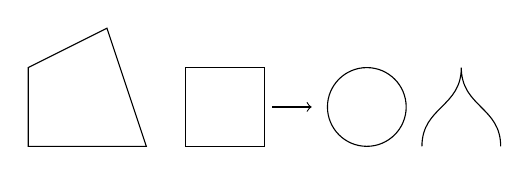
\begin{tikzpicture}
    \draw (0,0) -- (1.5,0) -- (1,1.5) -- (0,1) -- cycle;
    \draw (2,0) rectangle (3,1);
    \draw (4.3,0.5) circle (0.5cm);
    \draw [->] (3.1,0.5) -- (3.6,0.5);
    \draw (5,0) .. controls (5,0.5) and (5.5,0.5) .. (5.5,1)
        .. controls (5.5,0.5) and (6,0.5) ..(6,0);
\end{tikzpicture}
\end{minipage}
\hfill
\begin{minipage}{0.45\textwidth}
\begin{lstlisting}
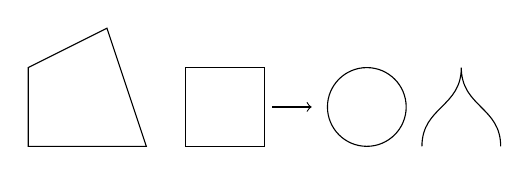
\begin{tikzpicture}
    \draw (0,0) -- (1.5,0) -- (1,1.5) -- (0,1) -- cycle;
    \draw (2,0) rectangle (3,1);
    \draw (4.3,0.5) circle (0.5cm);
    \draw [->] (3.1,0.5) -- (3.6,0.5);
    \draw (5,0) .. controls (5,0.5) and (5.5,0.5) .. (5.5,1)
        .. controls (5.5,0.5) and (6,0.5) ..(6,0);
\end{tikzpicture}
\end{lstlisting}
\end{minipage}
\end{figure}
 

Most drawings begins with \verb|\draw (x0,y0);| which decides the very first point of your drawing.
From there you can assign coordinates to link lines, or use keywords that create circles, ellipses, arcs, rectangles, etc, each with their own special syntax.
The syntax for \texttt{rectangle} uses the position of two opposite vertices: \verb|(3,0) rectangle (4,1)|.
On the other hand, \texttt{circle} takes the coordinates for the centre and a radius in either \texttt{cm}, \texttt{in}, \texttt{pt} or \texttt{em}.
If you are not quite sure what these units mean, just stick to \texttt{cm}.

The creation of arrows is just as straightforward, with using the option \verb|[->]| or \verb|[<-]| to indicate the orientation of the arrow.
Curved paths have a far more complicated syntax, using \texttt{controls}:
\begin{lstlisting}
(starting coordinate) .. controls (first control point) and (second control point) .. (end point)
\end{lstlisting}

Now imagine when you have to change the position of one of the drawings. What a nightmare!
For this reason, we have access to nodes --- portions of a picture that are given a position, shape and other options.
A \texttt{node} can be created at any coordinate in your drawing. One approach will be demonstrated now and another in the next section.
The basic syntax is the following:
\begin{lstlisting}
    \node [options] (name) at (x,y) {text in shape};
\end{lstlisting}

\begin{figure}[h]
\centering
\begin{minipage}{0.4\textwidth}
    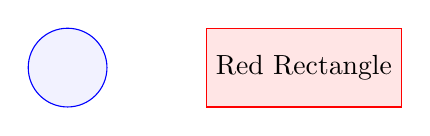
\begin{tikzpicture}
        \node [circle, draw=blue, fill=blue!5, minimum size=1cm,] (blueCircle) at (0,0) {};
        \node[rectangle, draw=red, fill=red!10, minimum height=1cm, minimum width = 2cm] (redRectangle) at (3,0) {Red Rectangle};
    \end{tikzpicture}
\end{minipage}
\hfill
\begin{minipage}{0.59\textwidth}
\begin{lstlisting}
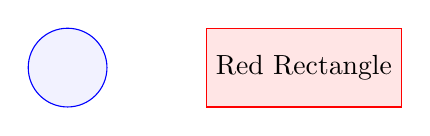
\begin{tikzpicture}
    \node [circle, draw=blue, fill=blue!5, minimum size=1cm,] (blueCircle) at (0,0) {};
    \node[rectangle, draw=red, fill=red!10, minimum height=1cm, minimum width = 2cm] () at (3,0) {Red Rectangle};
\end{tikzpicture}
\end{lstlisting}
\end{minipage}
\end{figure}

And not only can we use the names of the nodes place of coordinates, but we have access to both absolute and relative coordinates.
\begin{figure}[h]
    \centering
    \begin{minipage}{0.4\textwidth}
        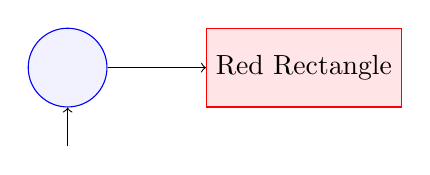
\begin{tikzpicture}
            \node [circle, draw=blue, fill=blue!5, minimum size=1cm,] (blueCircle) at (0,0) {};
            \node[rectangle, draw=red, fill=red!10, minimum height=1cm, minimum width = 2cm] (redRectangle) at (3,0) {Red Rectangle};
            \draw[->] (blueCircle) -- (redRectangle);
            \draw[->] (blueCircle) ++ (0,-1) -- (blueCircle);
        \end{tikzpicture}
    \end{minipage}
    \hfill
    \begin{minipage}{0.59\textwidth}
        \begin{lstlisting}
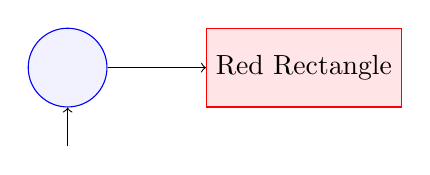
\begin{tikzpicture}
    \node [circle, draw=blue, fill=blue!5, minimum size=1cm,] (blueCircle) at (0,0) {};
    \node[rectangle, draw=red, fill=red!10, minimum height=1cm, minimum width = 2cm] (redRectangle) at (3,0) {Red Rectangle};
    \draw[->] (blueCircle) -- (redRectangle);
    \draw[->] (blueCircle) ++ (0,-1) -- (blueCircle);
\end{tikzpicture}
        \end{lstlisting}
    \end{minipage}
\end{figure}


\subsection{Control system}
For this upcoming section, please take a look at \texttt{Examples/Control-systems} for the examples in full.

\begin{figure}[h]\centering
    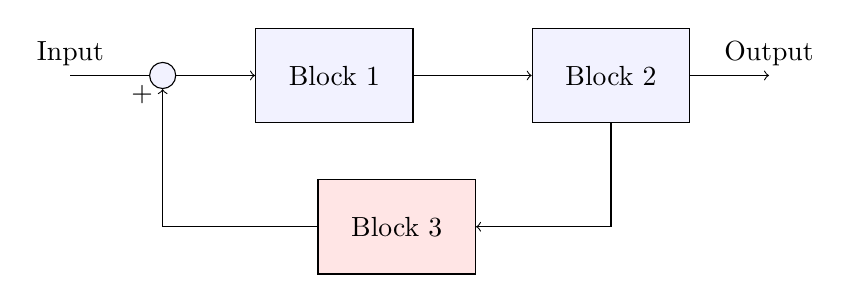
\begin{tikzpicture}
        %Blocks
        \node [block] (block1) at (0,0) {Block 1};
        \node [block, right = 1.5 cm of block1,] (block2) {Block 2};
        \node [block, below left = 1 cm of block2, fill=red!10] (block3) {Block 3} ;
        \node [sum, left = of block1] (sum1) {};
        %Arrows
        \draw[->] (block1) -- (block2);
        \draw[->] (block2.east) -- ++(1.0,0) node [right,above](){Output};
        \draw[->] (block2.south) |- (block3.east) ;
        \draw[->] (block3.west) -| (sum1) node[below left](){+};
        \draw[->] (sum1.west) ++ (-1,0) node[above](){Input}-- (sum1.west)
            (sum1.east) -- (block1.west)
        ;
    \end{tikzpicture}
    \caption{Simple control system}
\end{figure}

You are probably able to replicate this exact block, but having to repeat all of those instructions for several blocks that are identical would be tedious.
Gladly, \texttt{tikzstyle} as well as some tikz libraries give us some special features to both eliminate repetition and be very precise with our arrow and text positioning.
\begin{lstlisting}
\usepackage{tikz}
\usetikzlibrary{positioning,shapes,arrows}

%Control blocks shortcuts
\tikzstyle{block} = [draw, minimum width = 2cm, minimum height = 1.2cm, fill=blue!5]
\tikzstyle{sum} = [draw, fill=blue!5, circle, node distance=1cm]
\end{lstlisting}

\paragraph{Note:}
You can have a \texttt{tikzstyle} either inside one tikzpicture environment or for your entire document.
These are used commonly enough that the suggestion is to have them as a part of your entire document, as is the case in the templates. 

Now each block can be created by using the option \texttt{block}, instead of describing its minimum height, width and colour.
But we still have the option to overwrite the ``default'' colour if we want to.
Pay attention to absolute positioning on line 3, compared to relative positioning, as seen in lines 4, 5 and 6. 
\begin{figure}[h]\centering
    \begin{minipage}{0.44\textwidth}
    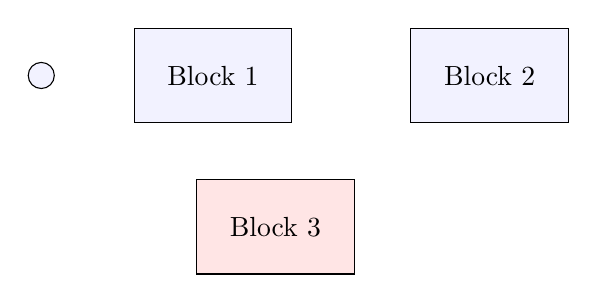
\begin{tikzpicture}
        %Blocks
        \node [block] (block1) at (0,0) {Block 1};
        \node [block, right = 1.5 cm of block1,] (block2) {Block 2};
        \node [block, below left = 1 cm of block2, fill=red!10] (block3) {Block 3} ;
        \node [sum, left = of block1] (sum1) {};
    \end{tikzpicture}
    \end{minipage}
    \hfill
    \begin{minipage}{0.55\textwidth}
        \begin{lstlisting}
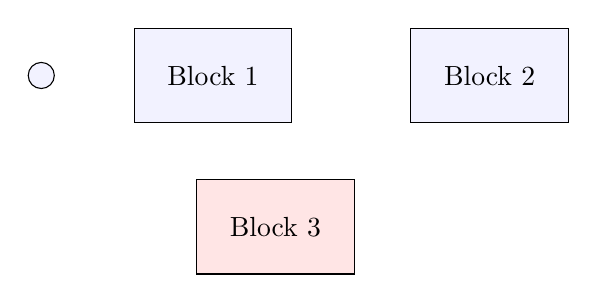
\begin{tikzpicture}
    %Blocks
    \node [block] (block1) at (0,0) {Block 1};
    \node [block, right = 1.5 cm of block1,] (block2) {Block 2};
    \node [block, below left = 1 cm of block2, fill=red!10] (block3) {Block 3} ;
    \node [sum, left = of block1] (sum1) {};
\end{tikzpicture}      
        \end{lstlisting}
    \end{minipage}
\end{figure}

Now we can add the arrows completely separately from the shapes.
And you will notice \verb!|-! and \verb!-|!, which create a \SI{90}{\degree} bend without the need to manually set the points.
\begin{figure}[h]
\centering
\begin{minipage}{0.45\textwidth}
    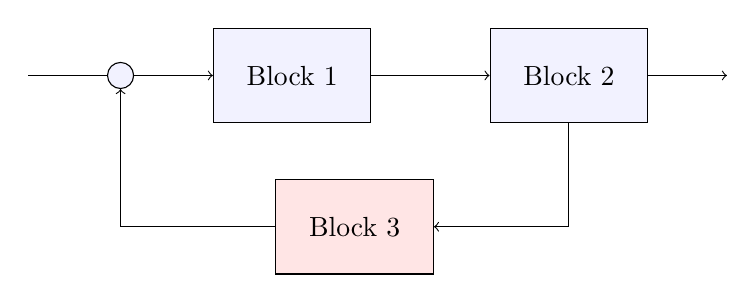
\begin{tikzpicture}
        %Blocks
        \node [block] (block1) at (0,0) {Block 1};
        \node [block, right = 1.5 cm of block1,] (block2) {Block 2};
        \node [block, below left = 1 cm of block2, fill=red!10] (block3) {Block 3} ;
        \node [sum, left = of block1] (sum1) {};
        %Arrows
        \draw[->] (block1) -- (block2);
        \draw[->] (block2.east) -- ++(1.0,0);
        \draw[->] (block2.south) |- (block3.east) ;
        \draw[->] (block3.west) -| (sum1) ;
        \draw[->] (sum1.west) ++ (-1,0) -- (sum1.west)
            (sum1.east) -- (block1.west)
        ;
    \end{tikzpicture}
\end{minipage}
\hfill
\begin{minipage}{0.45\textwidth}
\begin{lstlisting}
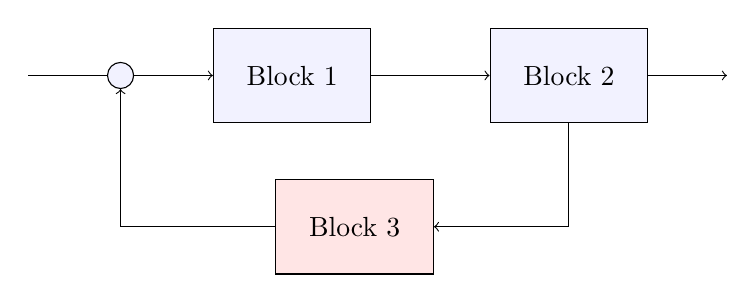
\begin{tikzpicture}
%Blocks
\node [block] (block1) at (0,0) {Block 1};
\node [block, right = 1.5 cm of block1,] (block2) {Block 2};
\node [block, below left = 1 cm of block2, fill=red!10] (block3) {Block 3} ;
\node [sum, left = of block1] (sum1) {};
%Arrows
\draw[->] (block1) -- (block2);
\draw[->] (block2.east) -- ++(1.0,0);
\draw[->] (block2.south) |- (block3.east) ;
\draw[->] (block3.west) -| (sum1) ;
\draw[->] (sum1.west) ++ (-1,0) -- (sum1.west)
    (sum1.east) -- (block1.west)
;
\end{tikzpicture}
\end{lstlisting}    
\end{minipage}
\end{figure}

Adding text in drawings requires a node, but gladly there is another way to create them.
Following a set of coordinates, we can simply start a node, like so:
\begin{figure}[h]\centering
\begin{minipage}{0.45\textwidth}
    \begin{tikzpicture}
        \draw[dashed] (0,1) -- (4,1) node[right](){text};
        \draw (0,0) node() {text 1} -- (4,0) node[above]() {text 2};
    \end{tikzpicture}
\end{minipage}
\hfill
\begin{minipage}{0.45\textwidth}
\begin{lstlisting}
\begin{tikzpicture}
    \draw[dashed] (0,1) -- (4,1) node[right](){text};
    \draw (0,0) node() {text 1} -- (4,0) node[above]() {text 2};
\end{tikzpicture}
\end{lstlisting}
\end{minipage}
\end{figure}

Finally we can combine all of this to create our control system.
\begin{lstlisting}
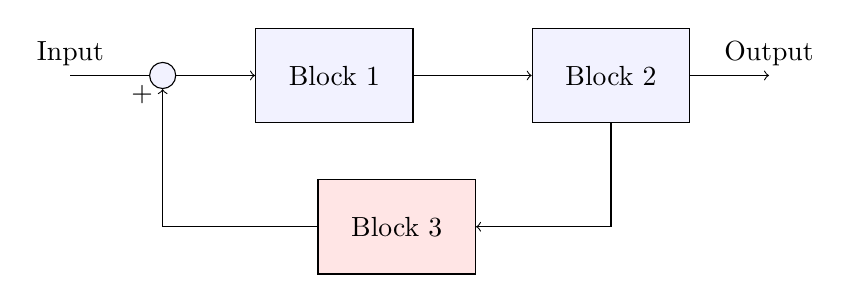
\begin{tikzpicture}
    %Blocks
    \node [block] (block1) at (0,0) {Block 1};
    \node [block, right = 1.5 cm of block1,] (block2) {Block 2};
    \node [block, below left = 1 cm of block2, fill=red!10] (block3) {Block 3} ;
    \node [sum, left = of block1] (sum1) {};
    %Arrows
    \draw[->] (block1) -- (block2);
    \draw[->] (block2.east) -- ++(1.0,0) node [right,above](){Output};
    \draw[->] (block2.south) |- (block3.east) ;
    \draw[->] (block3.west) -| (sum1) node[below left](){+};
    \draw[->] (sum1.west) ++ (-1,0) node[above](){Input}-- (sum1.west)
        (sum1.east) -- (block1.west)
    ;
\end{tikzpicture}
\end{lstlisting}
\begin{figure}[h]\centering
    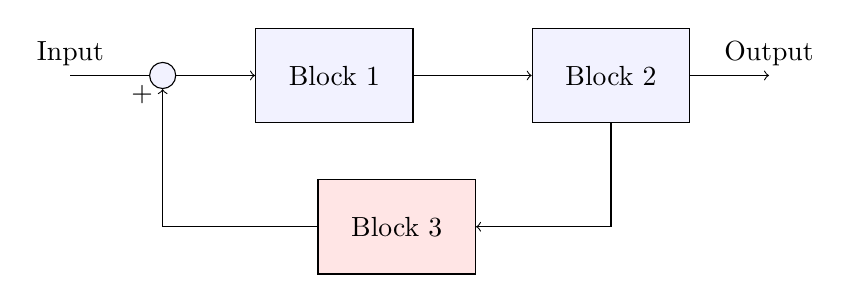
\begin{tikzpicture}
        %Blocks
        \node [block] (block1) at (0,0) {Block 1};
        \node [block, right = 1.5 cm of block1,] (block2) {Block 2};
        \node [block, below left = 1 cm of block2, fill=red!10] (block3) {Block 3} ;
        \node [sum, left = of block1] (sum1) {};
        %Arrows
        \draw[->] (block1) -- (block2);
        \draw[->] (block2.east) -- ++(1.0,0) node [right,above](){Output};
        \draw[->] (block2.south) |- (block3.east) ;
        \draw[->] (block3.west) -| (sum1) node[below left](){+};
        \draw[->] (sum1.west) ++ (-1,0) node[above](){Input}-- (sum1.west)
            (sum1.east) -- (block1.west)
        ;
    \end{tikzpicture}
\end{figure}